% Section 2 Header
\section{Fundamentals \& Big O}

\begin{frame}[c]{\empty}
    \begin{center}
        \Large\textbf{\secname}
    \end{center}
\end{frame}

% Slide 1: Concept
\begin{frame}{The Absolute Essentials}
  Before mastering coding patterns, you must master the fundamental building blocks.
  \begin{itemize}
    \item \textbf{Why?} Interviewers evaluate your ability to select the right tool for the job.
    \item \textbf{Key Areas:}
      \begin{itemize}
        \item Analyzing efficiency (Big O Complexity).
        \item Choosing the right data structures.
        \item Writing idiomatic, clean code under pressure.
      \end{itemize}
  \end{itemize}
\end{frame}

% Slide 2: Time & Space Complexity
\begin{frame}{Big O Notation Demystified}
  \begin{columns}
    \begin{column}{0.6\textwidth}
      How does the runtime or space requirement grow as input size $N$ increases?
      \begin{itemize}
        \item \textbf{Time Complexity:} Count dominant operations.
          \begin{itemize}
            \scriptsize
            \item $O(1)$ - Constant time.
            \item $O(\log N)$ - Logarithmic (halving search space).
            \item $O(N)$ - Linear (single pass).
            \item $O(N \log N)$ - Linearithmic (sorting).
            \item $O(N^2)$ - Quadratic (nested loops).
          \end{itemize}
        \item \textbf{Space Complexity:} Measure auxiliary memory (call stack, maps, arrays).
      \end{itemize}
    \end{column}
    \begin{column}{0.4\textwidth}
      \centering
      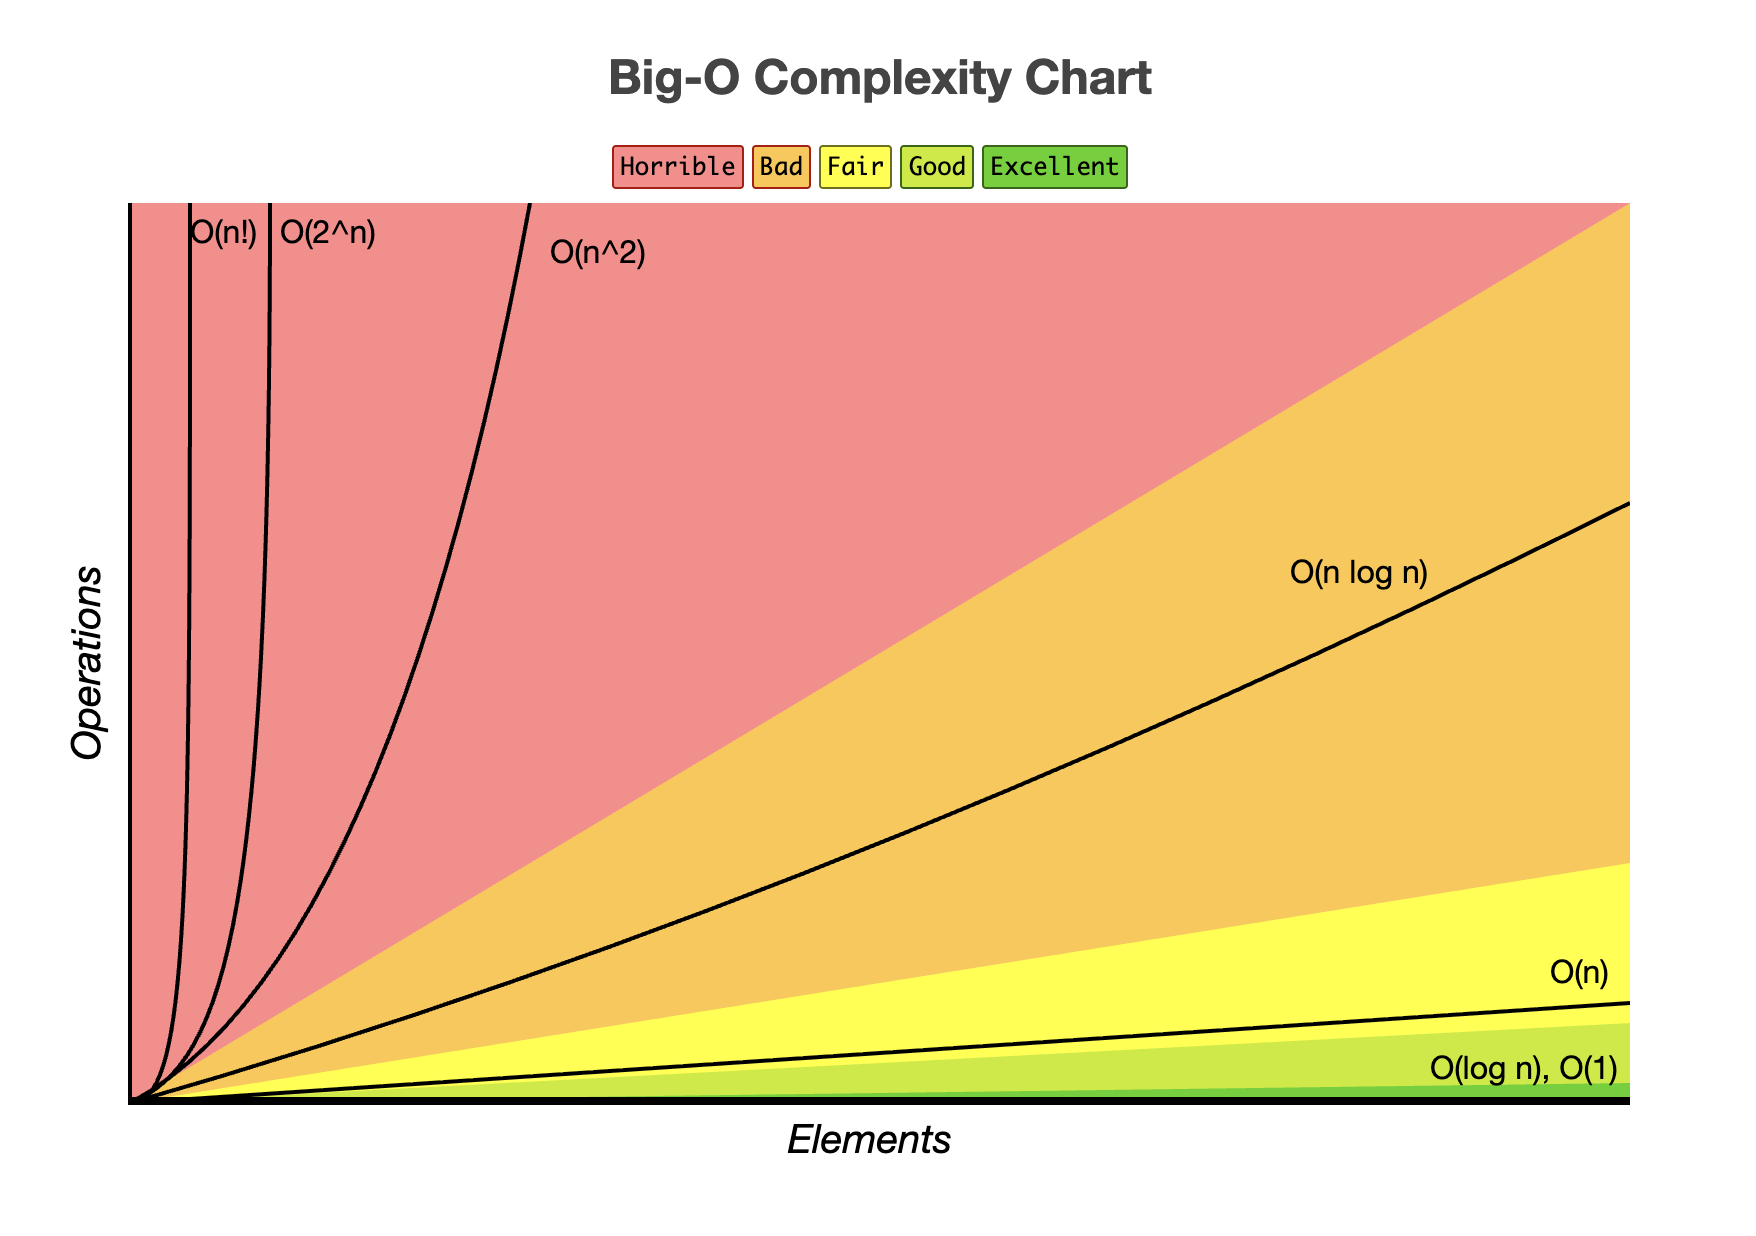
\includegraphics[width=\textwidth]{../bigO.png} \\
      \vspace{0.2cm}
      \tiny \href{https://www.bigocheatsheet.com/}{bigocheatsheet.com}
    \end{column}
  \end{columns}
\end{frame}

% Slide 2b: Complexity at N = 1,000,000
\begin{frame}{Growth Rates in Action ($N = 1,000,000$)}
  What do these complexities mean in practice for 1 million input elements?
  \vspace{0.3cm}
  \begin{table}[]
    \small
    \begin{tabular}{lll}
        \toprule
        \textbf{Complexity} & \textbf{Operations ($N = 10^6$)} & \textbf{Approx. Time (1GHz CPU)} \\ \midrule
        $O(1)$ & $1$ & $\approx 1$ ns (Instant) \\
        $O(\log N)$ & $\approx 20$ & $\approx 20$ ns (Instant) \\
        $O(N)$ & $1,000,000$ & $\approx 1$ ms (Instant) \\
        $O(N \log N)$ & $\approx 2 \times 10^7$ & $\approx 20$ ms (Instant) \\
        $O(N^2)$ & $10^{12}$ & $\approx 16.7$ minutes (\textbf{Timeout}) \\
        $O(2^N)$ & $2^{1,000,000}$ & $\gg$ Age of the Universe (\textbf{Impossible}) \\
        \bottomrule
    \end{tabular}
  \end{table}
\end{frame}

% Slide 3: Data Structures Crash Course
\begin{frame}{Data Structures Crash Course}
  \begin{table}[]
    \scriptsize
    \begin{tabular}{lll}
        \toprule
        \textbf{Data Structure} & \textbf{Strengths} & \textbf{Common Use Case} \\ \midrule
        \textbf{Array / List} & Fast index access ($O(1)$) & Ordered traversal, sorting \\
        \textbf{HashMap / Map} & Key lookup ($O(1)$ average) & Frequency counting, cache \\
        \textbf{HashSet / Set} & Duplicate removal, search ($O(1)$) & Visited trackers, unique items \\
        \textbf{Queue / Deque} & FIFO ordering ($O(1)$ push/pop) & BFS, level order traversal \\
        \bottomrule
    \end{tabular}
  \end{table}
\end{frame}

% Slide 4: Idiomatic Code
\begin{frame}{Writing Idiomatic Code under Pressure}
  Write production-ready, readable code rather than terse competitive code.
  \begin{itemize}
    \item \textbf{Kotlin Idioms:}
      \begin{itemize}
        \item Use `maxOf(a, b)` and `minOf(a, b)` instead of custom ifs.
        \item Prefer `when` expressions for clean decision branches.
        \item Avoid force-unwrapping nullables (`!!`) unless absolutely safe.
      \end{itemize}
    \item \textbf{Self-Documentation:} Use descriptive variable names (`left`, `right`, `charCount`) instead of obscure ones (`l`, `r`, `c`).
  \end{itemize}
\end{frame}
